\section{Bases de datos distribuidas con SQL (CITUS Data)}

Para esta parte de la práctica decidimos crear el clúster sobre máquinas reales y no sobre la máquina virtual, para profundizar en detalles acerca de cómo configurar PostgreSQL en un entorno real, tanto a la hora de permitir conexiones desde el exterior como habilitar la autenticación y la conexión entre nodos de un clúster.

\subsection*{Preparación}

Las máquinas que alquilamos en la nube de OVH son servidores con 1 vCore, 2 GB de RAM y 20 GB de almacenamiento SSD corriendo Ubuntu 22.04, su oferta más económica. Para la conexión a estas máquinas optamos por la autenticación mediante clave pública/privada. Para ello debemos generar un par de claves dentro del directorio \texttt{\$HOME/.ssh} de nuestra máquina local, esto lo hacemos mediante el comando:
\begin{verbatim}
ssh-keygen -b 4096 -f ~/.ssh/keys/ovh
\end{verbatim}

Esto nos genera la clave privada que guardaremos en nuestra máquina y una clave pública que usaremos a la hora de configurar las máquinas en el portal de OVH. Para facilitar el trabajo contra estas máquinas, definimos en nuestra máquina local en la ruta \$HOME/.ssh/config el siguiente archivo de configuración:

\begin{minted}[frame=single, fontsize=\footnotesize]{sh}
Host ovh*
  User      ubuntu
  IdentityFile ~/.ssh/keys/ovh

Host ovh1
  HostName  51.210.241.66

Host ovh2
  HostName  51.210.241.239

Host ovh3
  HostName  51.210.241.207
\end{minted}

Gracias a este, podremos conectarnos mediante \texttt{ssh} a las máquinas sin tener que escribir el usuario o la dirección IP pública de las máquinas, ya que podremos usar \texttt{ssh ovh1}, por ejemplo. Finalmente, dentro de cada máquina, cambiamos su nombre mediante el siguiente comando:
\begin{verbatim}
sudo hostnamectl hostname <nuevo_nombre>
\end{verbatim}

\subsection*{Instalación}

Para instalar PostgreSQL y su extensión Citus seguimos el \href{https://docs.citusdata.com/en/stable/installation/multi_node_debian.html#ubuntu-or-debian}{guion} de los propios creadores de Citus. Comenzamos creando el script bash \texttt{all\_nodes\_terraform.sh} que se deberá ejecutar en todas las máquinas:

\begin{minted}[frame=single, fontsize=\footnotesize]{sh}
#!/bin/bash

# ejecutar desde local: ssh user@host 'bash -s' < <path_to_this_file>

POSTGRES_PASSWORD="***"

# Añadir el repositorio de Citus al empaquetador de Ubuntu
curl https://install.citusdata.com/community/deb.sh | sudo bash

# Instalar Postgres y Citus
sudo apt-get -y install postgresql-16-citus-12.1

# Precargar la extensión Citus
sudo pg_conftool 16 main set shared_preload_libraries citus

# Iniciar el servicio de Postgres y habilitarlo para arrancar al iniciar
sudo systemctl start postgresql
sudo systemctl enable postgresql

# Modificamos la contraseña del usuario postgres
sudo -i -u postgres psql -c "ALTER USER postgres WITH PASSWORD '${POSTGRES_PASSWORD}';"

# Modificamos el archivo /etc/postgres/16/main/postgresql.conf mediante comando
sudo pg_conftool 16 main set listen_addresses '*'

# Al archivo pg_hba.conf de nuestra versión instalada añadimos la siguiente línea
# que otorga acceso completo a usuarios autentificados
echo -e "\n# Allow access from all IP addresses\nhost   all     all     0.0.0.0/0      md5" 
| sudo tee -a /etc/postgresql/16/main/pg_hba.conf

# Reiniciamos el servicio de postgres
sudo systemctl restart postgresql

# Los diferentes nodos del clúster deben de poder comunicarse entre sí
# Para ello, creamos el archivo .pgpass en el directorio $HOME del usuario postgres
# Postgres leerá de ese archivo las contraseñas de distintas conexiones
# Usamos * para indicarle que use la misma contraseña para todas las conexiones, desde cada nodo a los otros 2
# https://docs.citusdata.com/en/v8.3/admin_guide/cluster_management.html#increasing-worker-security
sudo bash -c "echo '*:*:*:*:${POSTGRES_PASSWORD}' > /var/lib/postgresql/.pgpass"

# Cambiamos permisos de lectura y escritura únicamente para el usuario postgres
sudo chown postgres:postgres /var/lib/postgresql/.pgpass
sudo chmod 600 /var/lib/postgresql/.pgpass
\end{minted}

Con este script, instalamos PostgreSQL y Citus, configuramos PostgreSQL para escuchar tráfico en todas sus interfaces de red para poder enviar solicitudes desde internet y añadimos un nuevo tipo de conexión aceptada, desde cualquier dirección IP, pero que requiere de autentificación por contraseña. \\

Finalmente, acorde a la \href{https://docs.citusdata.com/en/v8.3/admin_guide/cluster_management.html#increasing-worker-security}{guía} de Citus acerca de cómo manejar la conexión entre nodos de un clúster, definimos el archivo \texttt{.pgpass} en la carpeta \texttt{\$HOME} del usuario postgres, creado cuando instalamos PostgreSQL. Este archivo es necesario para que los nodos se puedan comunicar entre sí, ya que, al no poder configurar las conexiones entre nodos en la misma red por limitaciones de nuestro proveedor cloud, estas conexiones también deberán ser autenticadas. \\

\noindent Para ejecutar este script en cada máquina, desde nuestra máquina local podemos hacer:
\begin{minted}[frame=single, fontsize=\footnotesize]{shell}
ssh username@host 'bash -s' <path_script.sh>
\end{minted}

\subsection*{Configurar Citus}

Una vez que tenemos PostgreSQL y Citus instalados y configurados a nivel de sistema, debemos configurar Citus. Las extensiones en PostgreSQL se asocian a una base de datos, por lo que podemos tener una base de datos llamada \texttt{citus} donde instalaremos la extensión mientras que el resto de bases de datos se comportarán como bases de datos PostgreSQL estándar. Para esto, creamos otro script, \texttt{all\_nodes\_citus.sh}, que se ejecutará en todas las máquinas del clúster:

\begin{minted}[frame=single, fontsize=\footnotesize]{shell}
# Eliminar extensión y base de datos citus
sudo -i -u postgres psql -d citus -c "DROP EXTENSION citus CASCADE;"
sudo -i -u postgres psql -c "DROP DATABASE citus;"

# Recrear base de datos citus
sudo -i -u postgres psql -c "CREATE DATABASE citus;"

# Añadir la extensión citus a la base de datos citus
sudo -i -u postgres psql -d citus -c "CREATE EXTENSION citus;"

# Verificamos que citus se ha instalado correctamente
sudo -i -u postgres psql -d citus -c "SELECT * FROM citus_version();"
\end{minted}

Finalmente, escogeremos una sola máquina para actuar como nodo coordinador, en nuestro caso, \texttt{ovh1}. En ella, deberemos ejecutar los comandos SQL para proclamar el nodo coordinador y añadir los demás nodos worker. Estos comandos SQL los tenemos recogidos en otro script, \texttt{coordinador\_citus.sh}, que solo se ejecutara en el nodo coordinador:

\begin{minted}[frame=single, fontsize=\footnotesize]{shell}
# Registrar la dirección del nodo coordinador
sudo -i -u postgres psql -d citus -c "SELECT citus_set_coordinator_host('51.210.241.66', 5432);"

# Añadir los nodos worker
sudo -i -u postgres psql -d citus -c "SELECT * from citus_add_node('51.210.241.239', 5432);"
sudo -i -u postgres psql -d citus -c "SELECT * from citus_add_node('51.210.241.207', 5432);"

# Verificar clúster
sudo -i -u postgres psql -d citus -c "SELECT * FROM citus_get_active_worker_nodes();"
\end{minted}

Después de ejecutar los scripts, obtenemos la salida mostrada en la figura \ref{fig:citus_cluster}, donde podemos observar que el clúster se ha creado correctamente.

\begin{figure}[H]
\centering
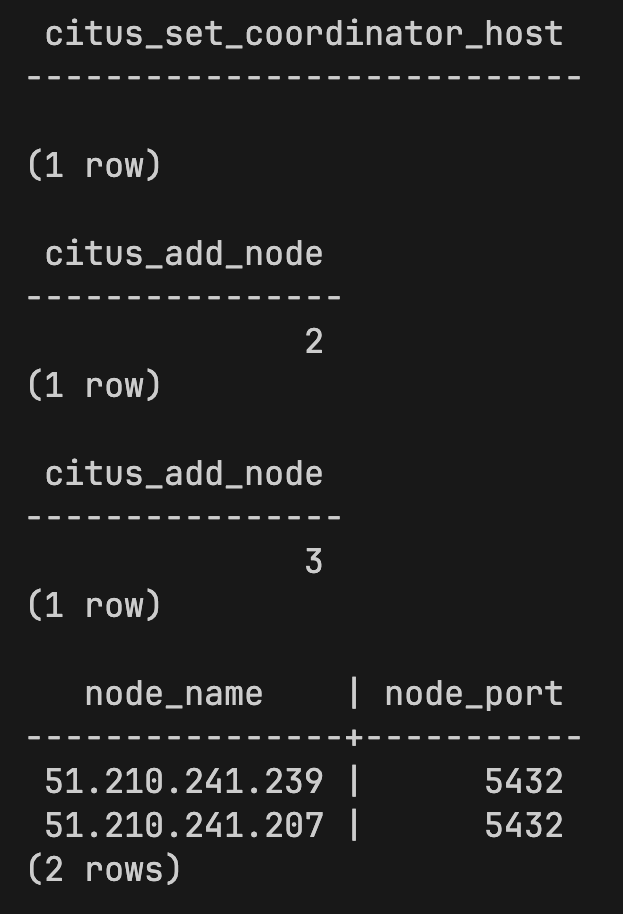
\includegraphics[width=0.27\textwidth]{fotos/citus/terraform.png}
\caption{Citus, cluster montado.}
\label{fig:citus_cluster}
\end{figure}


\subsection*{Trabajar contra el clúster}

En primer lugar se nos pide que, suponiendo que la base de datos crecerá al incorporar nuevos partidos de nuevas ediciones de torneos, distribuyamos los datos. La tabla de \texttt{partido} es la elección obvia para ser distribuida, particionando por el atributo \texttt{torneo}, lo cual nos garantiza que toda la información relacionada con los partidos en un torneo esté localizada en un único nodo. Esto minimiza las comunicaciones entre nodos y mejora el rendimiento de las consultas relacionadas con un torneo específico. Por extensión, la tabla \texttt{set\_partidos} irá co-localizada con \texttt{partido}, así como la tabla \texttt{edicion\_torneo}. Ambas también particionadas por el atributo \texttt{torneo}. \\

Las tablas \texttt{pais} y \texttt{torneo} las pondremos como tablas de referencia, esto es, tablas que son replicadas entre todos los nodos \texttt{worker} ya que son tablas pequeñas que no cambian con frecuencia. \\

Hacemos un inciso para mencionar que los nodos que almacenan datos son, principalmente, los \texttt{workers}, encargados de almacenar tablas distribuidas y de referencia. El nodo \texttt{coordinador} es el punto de entrada al clúster y se encarga de organizar las consultas y lanzarlas a los \texttt{workers} adecuados. No obstante, existen un tipo de tablas que sí pueden guardarse en el nodo \texttt{coordinador}: las tablas locales. Estas son tablas de PostgreSQL \textit{vanilla} que no han sido declaradas como distribuidas o de referencia. \\

Una vez que tenemos definido cómo vamos a distribuir los datos, cargamos el esquema de la primera parte del trabajo y le añadimos el siguiente código SQL para definir cómo manejaremos las tablas dentro de Citus:

\begin{minted}[frame=single, fontsize=\footnotesize]{sql}
-- Tablas de referencia (copiadas a todos los worker)
SELECT create_reference_table('pais');
SELECT create_reference_table('torneo');
SELECT create_reference_table('jugador');

-- Tablas distribuidas
SELECT create_distributed_table('partido', 'torneo');
SELECT create_distributed_table('edicion_torneo', 'torneo', colocate_with => 'partido');
SELECT create_distributed_table('sets_partido', 'torneo', colocate_with => 'partido');
SELECT create_distributed_table('ranking', 'jugador');
\end{minted}

\begin{figure}[H]
\centering
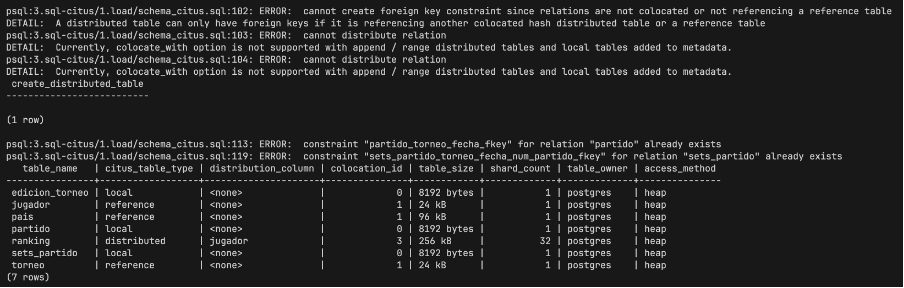
\includegraphics[width=0.9\textwidth]{fotos/citus/foreig_key_error.png}
\caption{Citus, error en claves foráneas.}
\label{fig:fk_citus}
\end{figure}

\noindent No obstante, de esta forma obtenemos el error mostrado en la figura \ref{fig:fk_citus}, en el que Citus nos indica que no puede añadir claves foráneas a la tabla distribuida de \texttt{partido}, porque las tablas distribuidas solo pueden tener claves foráneas que apunten a tablas de referencia o a una tabla distribuida co-localizada con la tabla que declara la clave foránea. \\

Como podemos observar, las tablas distribuidas relativas a los torneos no se han distribuido y se han quedado como tablas locales, su valor por defecto; este es el motivo por el cual no hemos podido añadir las claves foráneas. Para solventar esto y mantener las claves foráneas en nuestro esquema, debemos modificar el código de la siguiente manera:

\begin{minted}[frame=single, fontsize=\footnotesize]{sql}
DROP TABLE IF EXISTS pais CASCADE;
DROP TABLE IF EXISTS jugador CASCADE;
DROP TABLE IF EXISTS torneo CASCADE;
DROP TABLE IF EXISTS edicion_torneo CASCADE;
DROP TABLE IF EXISTS partido CASCADE;
DROP TABLE IF EXISTS sets_partido CASCADE;
DROP TABLE IF EXISTS ranking CASCADE;

CREATE TABLE pais (...);

CREATE TABLE jugador (...);

CREATE TABLE torneo (...);

CREATE TABLE edicion_torneo (...);

CREATE TABLE partido (...);

CREATE TABLE sets_partido (...);

CREATE TABLE ranking (...);

-- Tablas de referencia (copiadas a todos los worker)
SELECT create_reference_table('pais');
SELECT create_reference_table('torneo');
SELECT create_reference_table('jugador');

-- Tablas distribuidas
SELECT create_distributed_table('partido', 'torneo');
SELECT create_distributed_table('edicion_torneo', 'torneo', colocate_with => 'partido');
SELECT create_distributed_table('sets_partido', 'torneo', colocate_with => 'partido');
SELECT create_distributed_table('ranking', 'jugador');

-- Después de distribuir las tablas, podemos crear las claves foráneas de tablas distribuidas, no antes

-- Clave foránea para partido
ALTER TABLE partido 
ADD CONSTRAINT partido_torneo_fecha_fkey
FOREIGN KEY (torneo, fecha) 
REFERENCES edicion_torneo (torneo, fecha);

-- Clave foránea para sets_partido
ALTER TABLE sets_partido 
ADD CONSTRAINT sets_partido_torneo_fecha_num_partido_fkey
FOREIGN KEY (torneo, fecha, num_partido) 
REFERENCES partido (torneo, fecha, num_partido);
\end{minted}

En este código definimos las claves foráneas una vez que las tablas se han distribuido correctamente. De esta forma, no tenemos ningún fallo. Podemos observar cómo quedan nuestras tablas (figura \ref{fig:dist_citus}) mediante la instrucción:

\begin{minted}[frame=single, fontsize=\footnotesize]{sql}
SELECT * FROM citus_tables;
\end{minted}

\begin{figure}[H]
\centering
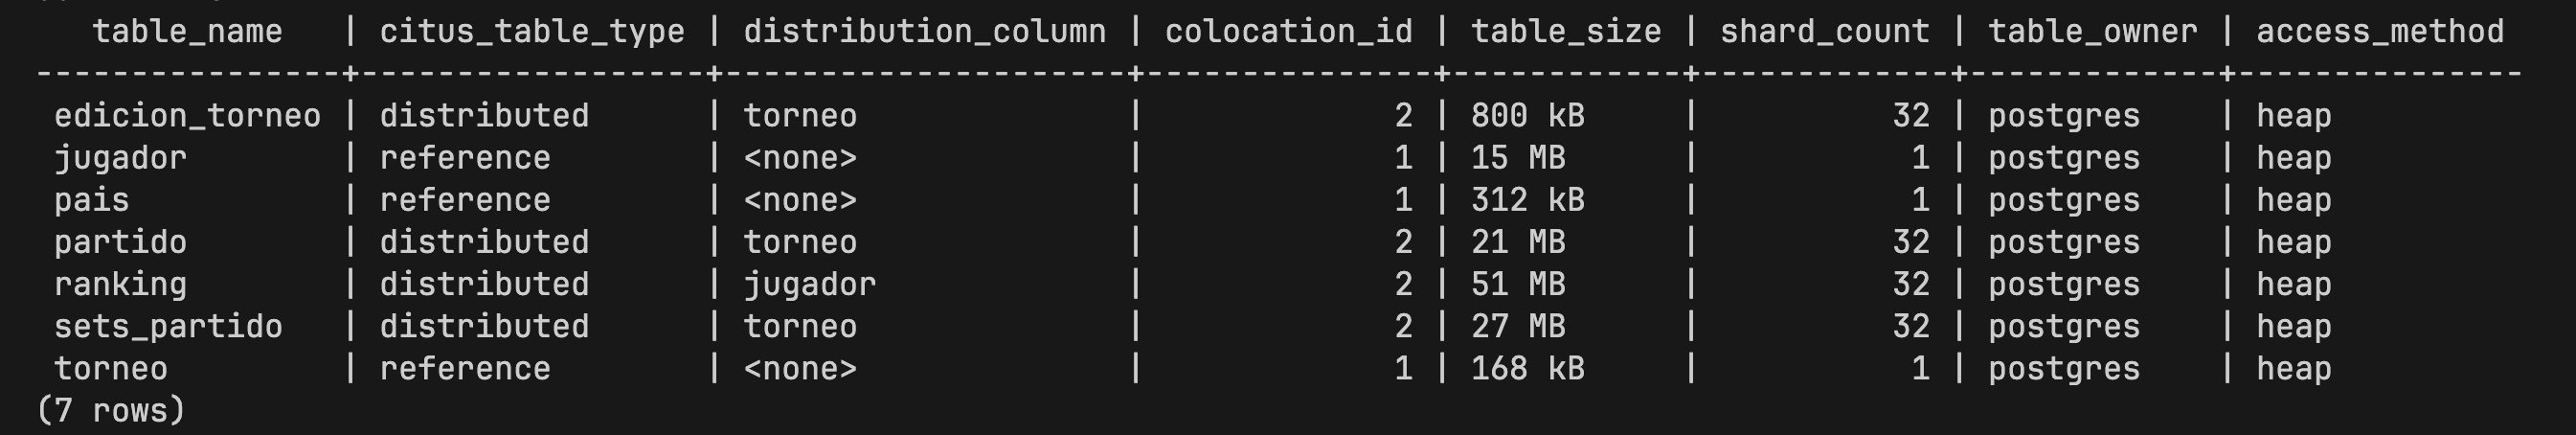
\includegraphics[width=0.9\textwidth]{fotos/citus/table_sizes_and_distributed.png}
\caption{Distribución final de tablas en Citus.}
\label{fig:dist_citus}
\end{figure}

En la figura \ref{fig:dist_citus} podemos observar cómo nuestras elecciones para las tablas distribuidas parecen acertadas si comparamos el tamaño en megas de las tablas distribuidas y en kilobytes de las de referencia. La única excepción a esto es la tabla \texttt{jugador}, que hemos dejado como tabla de referencia ya que, si la distribuyéramos, no podríamos co-localizarla con \texttt{partido}, y las consultas que unan \texttt{jugador} y \texttt{partido} (la mayoría), requerirían de transferencias entre nodos. Así, a pesar de que \texttt{jugador} es una tabla que previsiblemente aumentará a medida que nuevos jugadores entren en el circuito, es más eficiente no distribuirla y dejarla como tabla de referencia, ya que presuponemos que la tabla de \texttt{partido} crecerá más rápido que la de jugadores porque, por cada nuevo jugador, estos jugarán uno o más partidos.

\subsection*{Lanzar consultas al clúster}

Para enviar consultas al clúster desde nuestra máquina local podemos usar un cliente gráfico como DBeaver, ya que Citus es transparente a los clientes de PostgreSQL, dejándose ver como una base de datos PostgreSQL estándar. \\

También podemos utilizar \texttt{psql}, el cliente de PostgreSQL para la terminal. Para mejorar la ergonomía al usar esta herramienta, podemos definir dos ficheros en el directorio \texttt{\$HOME} de nuestra máquina local: \texttt{.pgpass}, que al igual que hicimos en los servidores, almacenará conjuntos de servidores:puerto:base\_datos:usuario:contraseña, y el archivo \texttt{.pg\_service.conf}, que nos permitirá poner un alias a las conexiones de PostgreSQL:

\begin{minted}[frame=single, fontsize=\footnotesize]{sh}
[tenis]
host=51.210.241.66
port=5432
dbname=tenis
user=postgres

[citus]
host=51.210.241.66
port=5432
dbname=citus
user=postgres

[citus-worker-1]
host=51.210.241.239
port=5432
dbname=citus
user=postgres

[citus-worker-2]
host=51.210.241.207
port=5432
dbname=citus
user=postgres
\end{minted}

Así, desde nuestra máquina local, podemos lanzar consultas SQL definidas en archivos \texttt{.sql} de forma muy cómoda con el siguiente comando:

\begin{minted}[frame=single, fontsize=\footnotesize]{sh}
psql service=[service_name] -f <path_to_sql_file>
\end{minted}

No comentaremos la semántica del código de las propias consultas, al ser idéntico al descrito en el primer apartado (modelo relacional). Los resultados de las mismas también coinciden con los mostrados en ese apartado, y pueden verse en las figuras \ref{fig:q1_citus}, \ref{fig:q2_citus}, \ref{fig:q3_citus}, \ref{fig:q4_citus} y \ref{fig:q5_citus}.

\subsubsection{Muestra todos los ganadores del torneo ``Wimbledon'' (Nombre apellidos y año). Ordena el resultado por año.}

\begin{minted}[frame=single, fontsize=\footnotesize]{sql}
select j.nombre, j.apellido, extract(year from p.fecha) as ano
from jugador j, partido p, torneo t
where j.id = p.ganador 
  and t.id = p.torneo 
  and t.nombre = 'Wimbledon' 
  and p.ronda = 'F'
order by ano
\end{minted}
\begin{figure}[H]
\centering
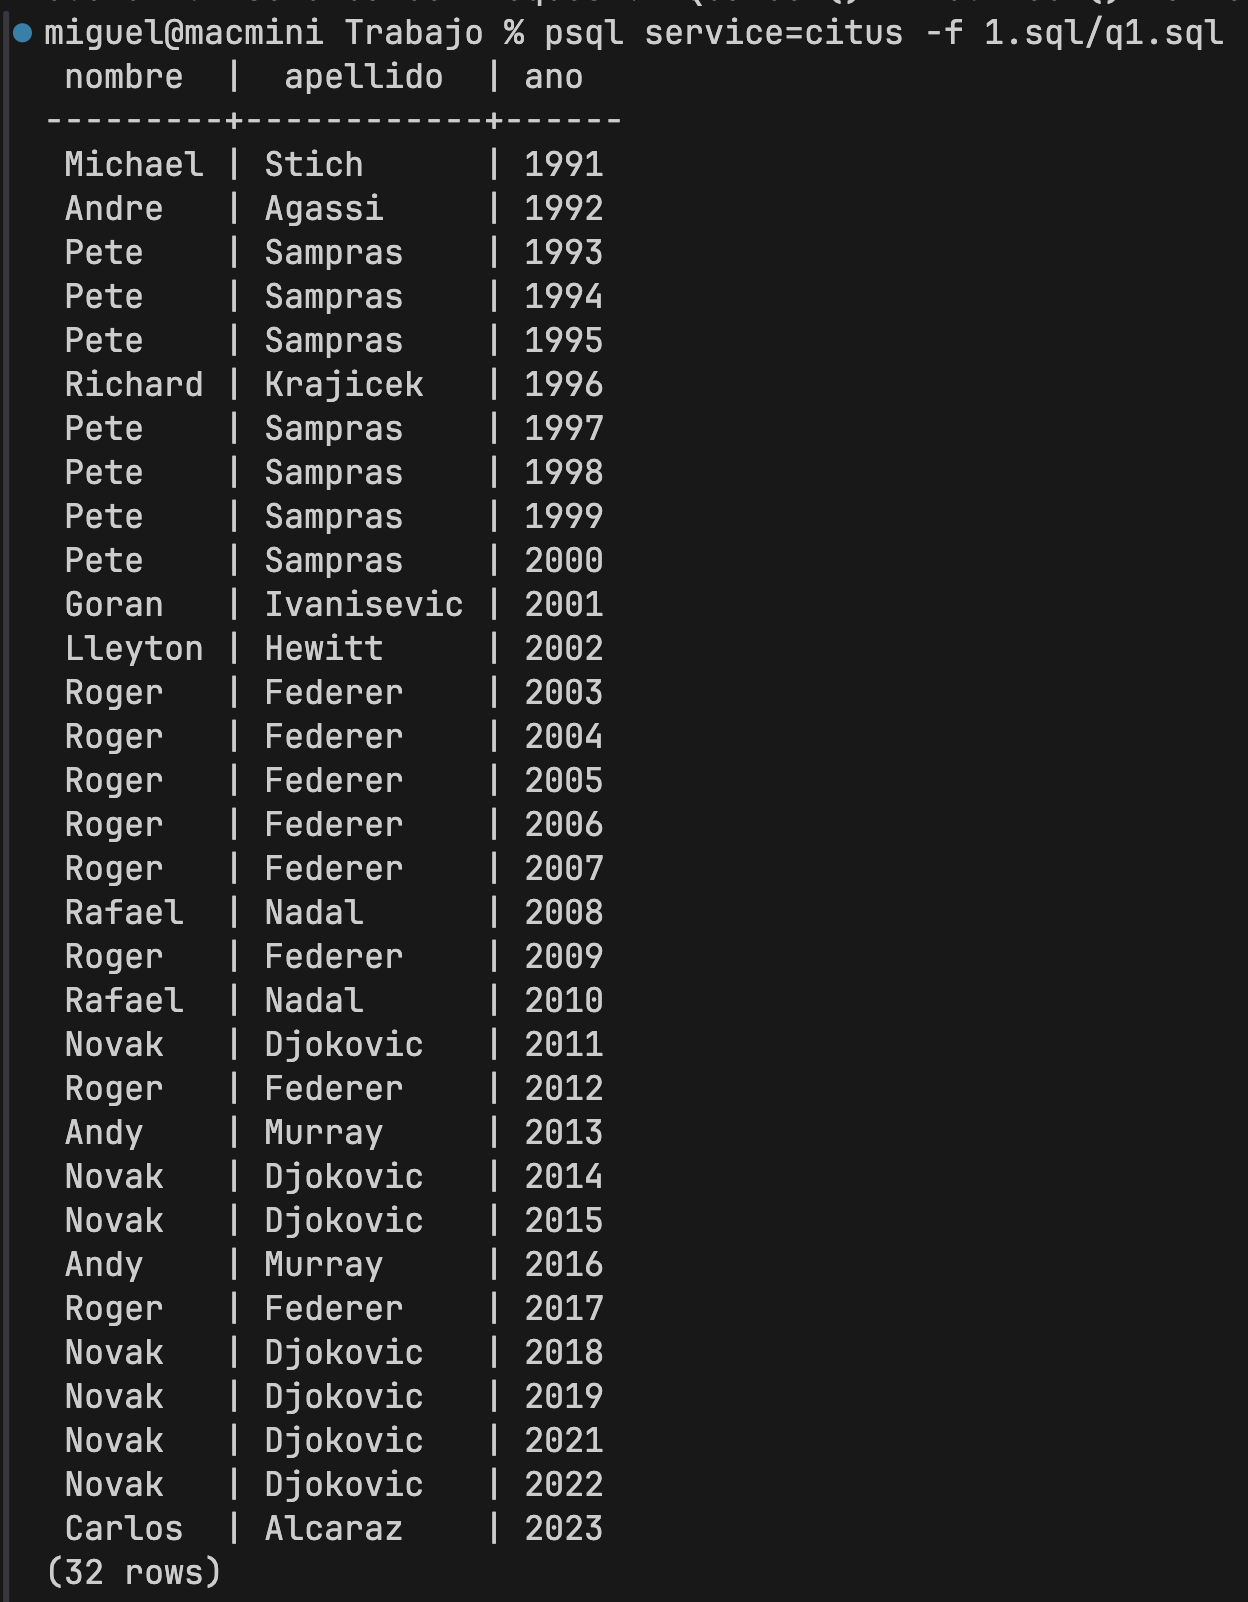
\includegraphics[width=0.4\textwidth]{fotos/citus/q1.png}
\caption{Bases de datos distribuidas. Citus, consulta 1.}
\label{fig:q1_citus}
\end{figure}


\subsubsection{Muestra los años en los que Roger Federer ganó algún torneo de nivel Gran Slam (G) o Master 1000 (M). Para cada año, muestra el número de torneos y lista sus nombres (ordenados por la fecha de celebración). Ordena el resultado por el año}

\begin{minted}[frame=single, fontsize=\footnotesize]{sql}
select extract(year from et.fecha) as ano, count(distinct t.id) as numero_torneos, 
	string_agg(t.nombre, ', ' order by et.fecha) as torneos
from jugador j, partido p, torneo t, edicion_torneo et
where j.id = p.ganador
  and t.id = et.torneo
  and p.torneo = t.id
  and p.fecha = et.fecha
  and p.ronda = 'F'
  and j.nombre = 'Roger'
  and j.apellido = 'Federer'
  and et.nivel in ('G', 'M')
group by ano
order by ano
\end{minted}

\begin{figure}[H]
\centering
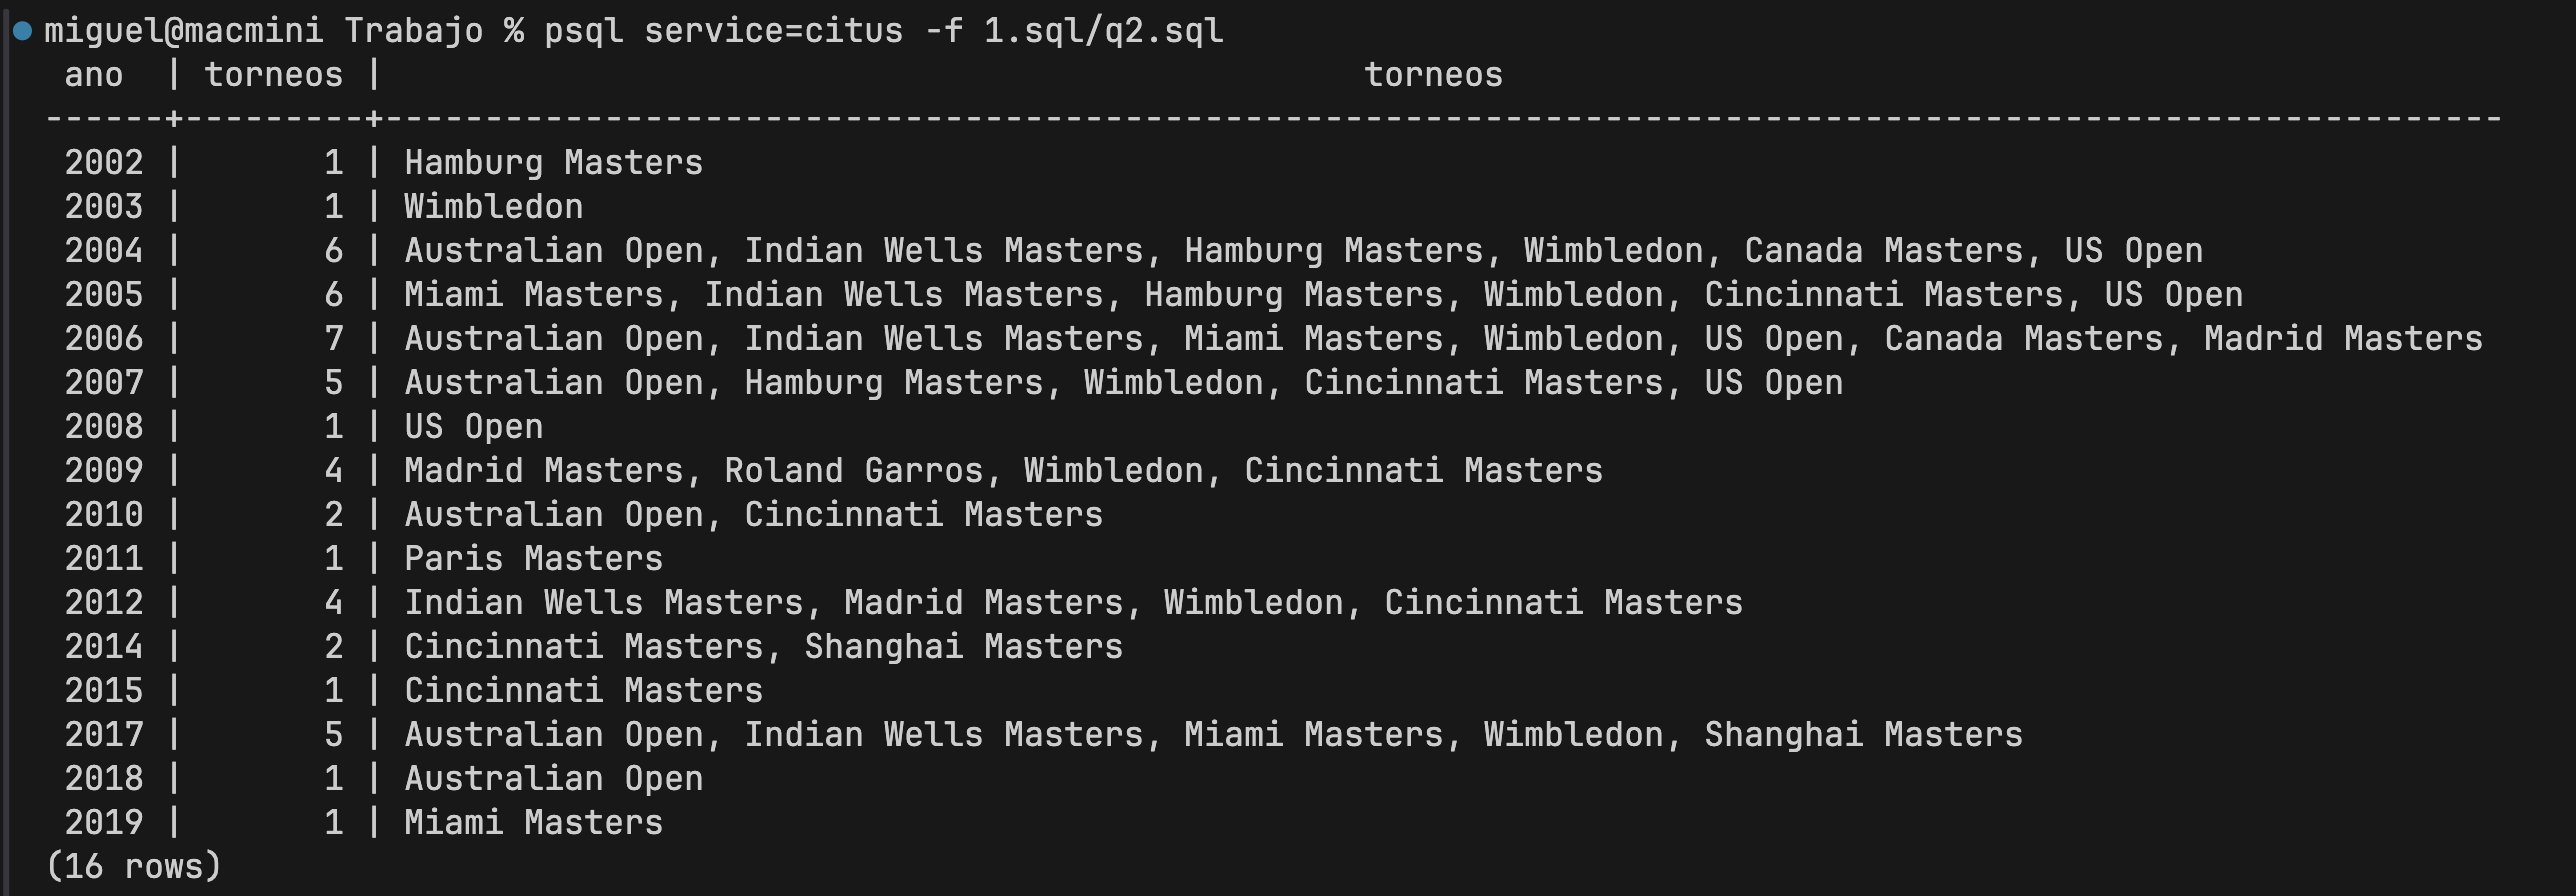
\includegraphics[width=0.7\textwidth]{fotos/citus/q2.png}
\caption{Bases de datos distribuidas. Citus, consulta 2.}
\label{fig:q2_citus}
\end{figure}




\subsubsection{Muestra los partidos de semifinales (ronda='SF') y final (ronda = 'F') del torneo de "Roland Garros" del 2018. Para cada partido muestra la ronda, el tipo de desenlace, el nombre y apellidos del ganador y el nombre y apellidos del perdedor y el resultado con el número de juegos del ganador y del perdedor en cada set, y opcionalmente en paréntesis el número de juegos del perdedor en el tie break}

\begin{minted}[frame=single, fontsize=\footnotesize]{sql}
select p.ronda, p.desenlace, jg.nombre || ' ' || jg.apellido AS ganador, 
	jp.nombre || ' ' || jp.apellido AS perdedor, 
	STRING_AGG(sp.juegos_ganador || '-' || sp.juegos_perdedor ||
		case
		  when sp.puntos_tiebreak_perdedor is not null then 
		  	'(' || sp.puntos_tiebreak_perdedor || ')'
		  else 
		  	'' 
		end, ', ' order by sp.num_set) as resultado
from partido p, jugador jg, jugador jp, sets_partido sp, torneo t
where jg.id = p.ganador
  and jp.id = p.perdedor
  and p.fecha = sp.fecha
  and p.num_partido = sp.num_partido
  and t.id = p.torneo
  and p.ronda in ('SF', 'F')
  and t.nombre = 'Roland Garros'
  and extract(year from p.fecha) = '2018'
group by p.ronda, p.desenlace, jg.nombre, jg.apellido, jp.nombre, jp.apellido
\end{minted}

\begin{figure}[H]
\centering
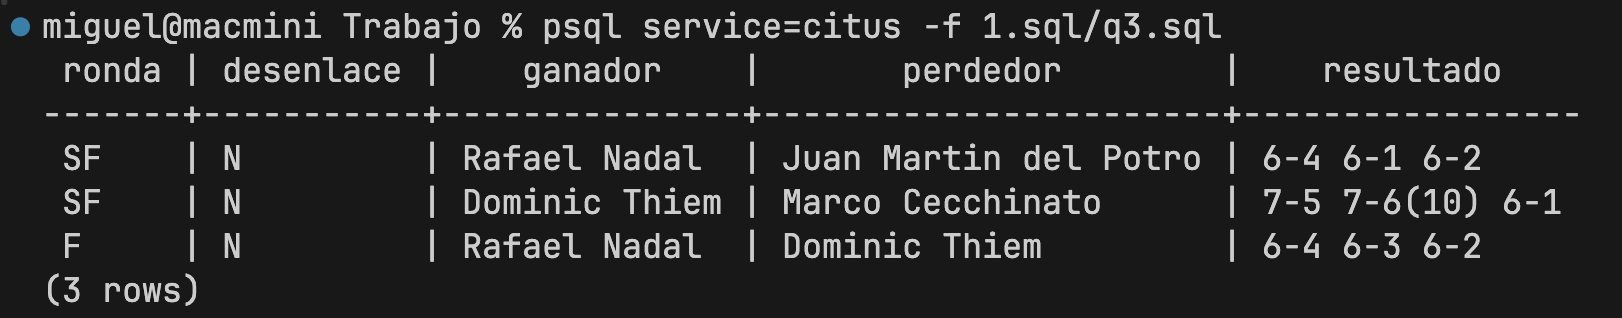
\includegraphics[width=0.7\textwidth]{fotos/citus/q3.png}
\caption{Bases de datos distribuidas. Citus, consulta 3.}
\label{fig:q3_citus}
\end{figure}




\subsubsection{Muestra la lista de jugadores españoles (ES) que ganaron algún torneo de nivel Gran Slam (G). Para cada jugador muestra los siguientes datos resumen de todos sus partidos: número de partidos jugados, porcentaje de victorias, porcentaje de aces, porcentaje de dobles faltas, porcentaje de servicios ganados, porcentaje de restos ganados, porcentaje de break points salvados (de los sufridos en contra), porcentaje de break points ganados (de los provocados a favor)}

\begin{minted}[frame=single, fontsize=\footnotesize]{sql}
with jugadores_espanoles_ganadores as (
    select distinct j.id as id_jugador, j.nombre || ' ' || j.apellido as jugador
    from partido p, jugador j, edicion_torneo et 
    where p.ganador = j.id 
        and p.torneo = et.torneo 
        and p.fecha = et.fecha
        and j.pais = 'ES'
        and p.ronda = 'F'
        and et.nivel = 'G'
)

select jeg.jugador, count(p.num_partido) as partidos,
    round(100.0 * sum(case when jeg.id_jugador = p.ganador then 1 else 0 end) / 
		count(p.num_partido), 1) as pcje_victorias, 
    round(100.0 * sum(case when jeg.id_jugador = p.ganador then 
		p.num_aces_ganador else p.num_aces_perdedor end) / 
        nullif(sum(case when jeg.id_jugador = p.ganador then p.num_ptos_servidos_ganador 
		else p.num_ptos_servidos_perdedor end), 0), 1) as pcje_aces, 
    round(100.0 * sum(case when jeg.id_jugador = p.ganador then p.num_dob_faltas_ganador 
		else p.num_dob_faltas_perdedor  end) / 
        nullif(sum(case when jeg.id_jugador = p.ganador then p.num_ptos_servidos_ganador 
		else p.num_ptos_servidos_perdedor end), 0), 1) as pcje_dobles_faltas, 
    round(100.0 * sum(case when jeg.id_jugador = p.ganador then 
		p.num_primeros_servicios_ganados_ganador + p.num_segundos_servicios_ganados_ganador 
        else p.num_primeros_servicios_ganados_perdedor + p.num_segundos_servicios_ganados_perdedor end) / 
        nullif(sum(case when jeg.id_jugador = p.ganador then p.num_ptos_servidos_ganador 
		else p.num_ptos_servidos_perdedor end), 0), 1) as pcje_servicios_ganados, 
    round(100.0 * sum(case when jeg.id_jugador = p.ganador then 
		p.num_ptos_servidos_perdedor - p.num_primeros_servicios_ganados_perdedor - 
		p.num_segundos_servicios_ganados_perdedor 
        else p.num_ptos_servidos_ganador - p.num_primeros_servicios_ganados_ganador - 
		p.num_segundos_servicios_ganados_ganador end) / 
        nullif(sum(case when jeg.id_jugador = p.ganador then p.num_ptos_servidos_perdedor 
		else p.num_ptos_servidos_ganador end), 0), 1) as pcje_restos_ganados,
    round(100.0 * sum(case when jeg.id_jugador = p.ganador then p.num_break_salvados_ganador 
		else p.num_break_salvados_perdedor end) / 
        nullif(sum(case when jeg.id_jugador = p.ganador then p.num_break_afrontados_ganador 
		else p.num_break_afrontados_perdedor end), 0), 1) as pcje_breaks_salvados, 
    round(100.0 * sum(case when jeg.id_jugador = p.ganador then 
		p.num_break_afrontados_perdedor - p.num_break_salvados_perdedor 
        else p.num_break_afrontados_ganador - p.num_break_salvados_ganador end) / 
        nullif(sum(case when jeg.id_jugador = p.ganador then p.num_break_afrontados_perdedor 
		else p.num_break_afrontados_ganador end), 0), 1) as pcje_breaks_ganados
from jugadores_espanoles_ganadores jeg, partido p
where jeg.id_jugador = p.ganador 
	or jeg.id_jugador = p.perdedor
group by jeg.jugador
\end{minted}

\begin{figure}[H]
\centering
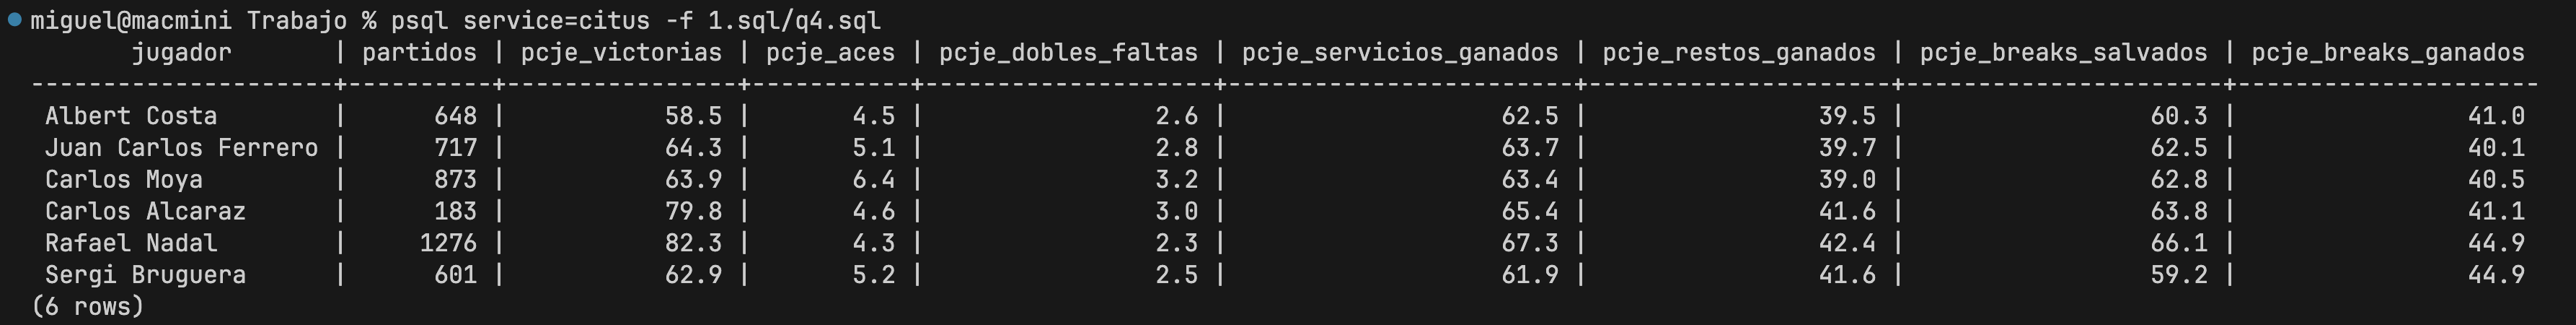
\includegraphics[width=0.9\textwidth]{fotos/citus/q4.png}
\caption{Bases de datos distribuidas. Citus, consulta 4.}
\label{fig:q4_citus}
\end{figure}




\subsubsection{Lista los jugadores que fueron derrotados (en algún partido del 2018) por el rival de Rafael Nadal de la primera ronda (R128) de Roland Garros de 2018}

\begin{minted}[frame=single, fontsize=\footnotesize]{sql}
with rival_nadal as (
	select case when jg.nombre = 'Rafael' then jp.id else jg.id end as id_jugador, 
		case when jg.nombre = 'Rafael' then jp.nombre || ' ' || jp.apellido 
		else jg.nombre || ' ' || jg.apellido end as jugador
	from partido p, jugador jg, jugador jp, edicion_torneo et, torneo t
	where p.ganador = jg.id 
		and p.perdedor = jp.id
		and p.torneo = et.torneo 
		and p.fecha = et.fecha
		and et.torneo = t.id 
		and t.nombre = 'Roland Garros'
		and p.ronda = 'R128'
		and extract(year from p.fecha) = '2018'
		and (jg.nombre = 'Rafael' and jg.apellido = 'Nadal' 
		or jp.nombre = 'Rafael' and jp.apellido = 'Nadal') 
)

select j.nombre || ' ' || j.apellido as jugador, j.pais as pais
from rival_nadal rn, partido p, jugador j
where rn.id_jugador = p.ganador 
	and p.perdedor = j.id
	and extract(year from p.fecha) = '2018'
\end{minted}

\begin{figure}[H]
\centering
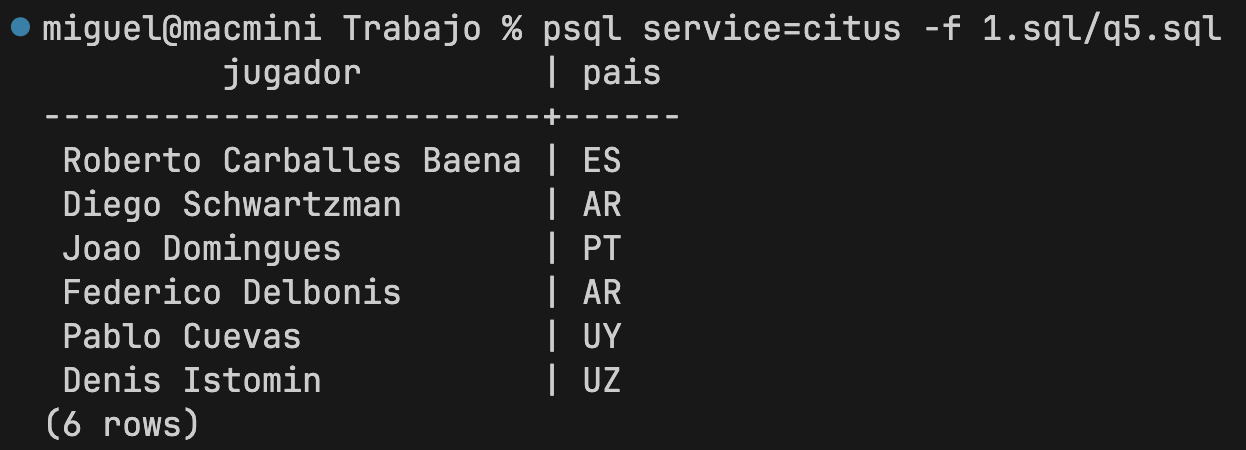
\includegraphics[width=0.65\textwidth]{fotos/citus/q5.png}
\caption{Bases de datos distribuidas. Citus, consulta 5.}
\label{fig:q5_citus}
\end{figure}




\subsection*{Factor de replicación}

En esta parte de la práctica se nos pide eliminar uno de los nodos para comprobar si Citus es capaz de ejecutar consultas con normalidad. Podemos parar un nodo \textit{worker} deteniendo el servicio de \texttt{postgres} mediante:

\begin{minted}[frame=single, fontsize=\footnotesize]{bash}
sudo systemctl stop postgres 
\end{minted}

Probamos ahora a enviar consultas y, como podemos ver en la figura \ref{fig:citus_worker_down} para una consulta a una tabla distribuida, el nodo coordinador detecta que un nodo \textit{worker} no responde y la consulta falla. Pero en la figura \ref{fig:citus_worker_down_but_reference} podemos observar como consultas a tablas de referencia siguen funcionando, ya que se pueden recuperar los datos.

\begin{figure}[H]
\centering
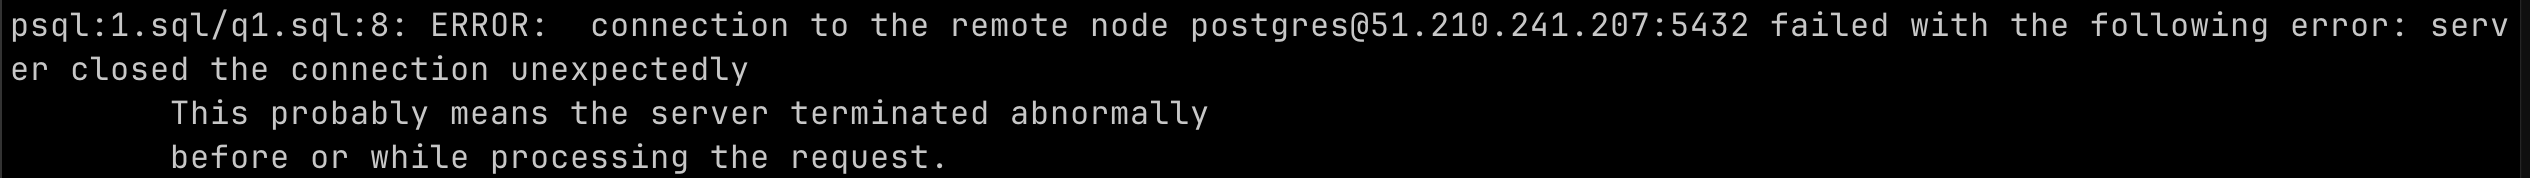
\includegraphics[width=0.8\textwidth]{fotos/citus/one_down_error.png}
\caption{Citus, error sin un nodo worker a tabla distribuida.}
\label{fig:citus_worker_down}
\end{figure}

\begin{figure}[H]
\centering
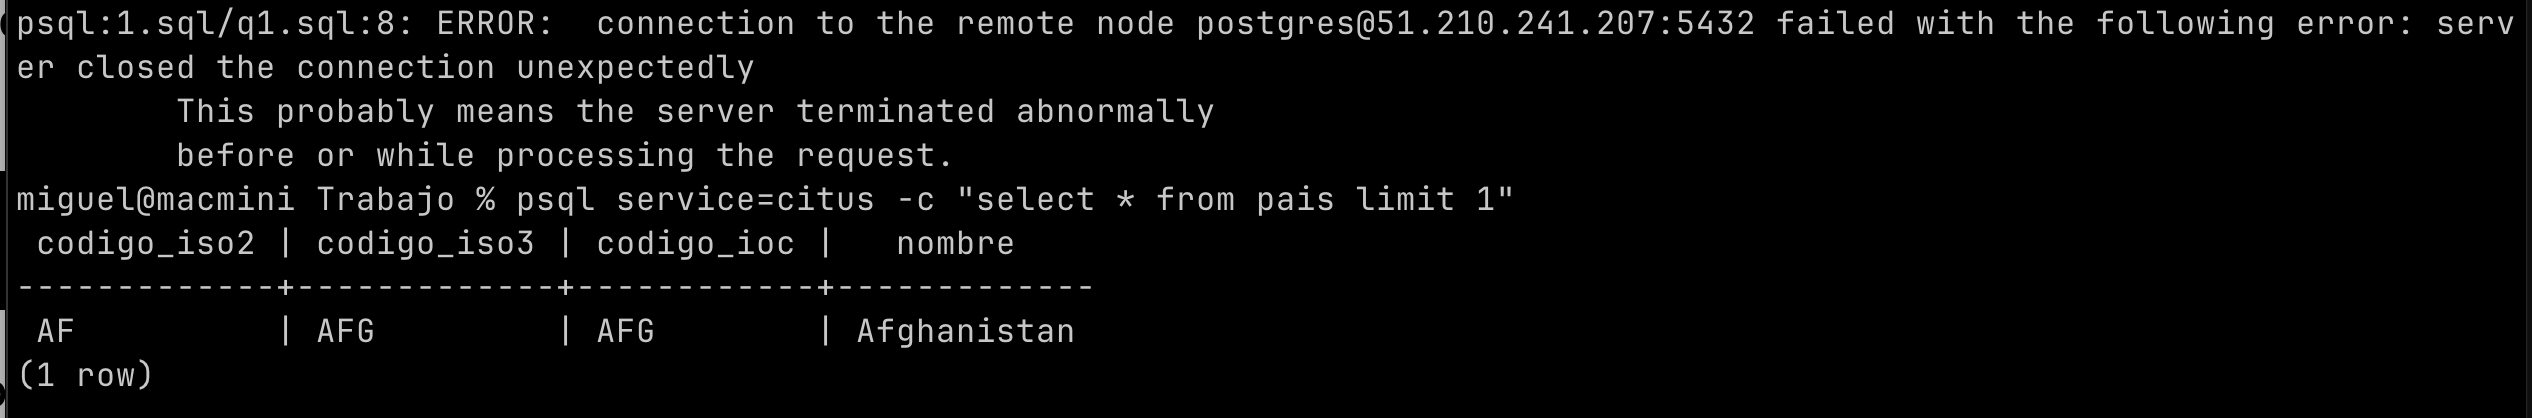
\includegraphics[width=0.8\textwidth]{fotos/citus/one_down_error_but_no.png}
\caption{Citus, consulta sin un nodo worker a tabla de referencia.}
\label{fig:citus_worker_down_but_reference}
\end{figure}

Para conseguir que las consultas a tablas distribuidas funcionen con nodos del \textit{cluster} no operativos, podemos modificar la variable \texttt{citus.shard\_replication\_factor}, que controla cuántas réplicas de cada fragmento o \textit{shard} se crean en diferentes nodos, asegurando que los datos estén disponibles incluso si un nodo falla. Para cambiar esta variable, debemos \textit{setear} en nuestro esquema esta variable de configuración antes de definir las tablas:

\begin{minted}[frame=single, fontsize=\footnotesize]{sql}
DROP TABLE IF EXISTS pais CASCADE;
DROP TABLE IF EXISTS jugador CASCADE;
DROP TABLE IF EXISTS torneo CASCADE;
DROP TABLE IF EXISTS edicion_torneo CASCADE;
DROP TABLE IF EXISTS partido CASCADE;
DROP TABLE IF EXISTS sets_partido CASCADE;
DROP TABLE IF EXISTS ranking CASCADE;

SET citus.shard_replication_factor = 2;

CREATE TABLE pais (
    codigo_iso2     CHAR(2)         PRIMARY KEY,
    codigo_iso3     CHAR(3)         UNIQUE NOT NULL,
    codigo_ioc      CHAR(3)         UNIQUE,
    nombre          VARCHAR(100)    UNIQUE NOT NULL
);

...
\end{minted}

\begin{figure}[H]
\centering
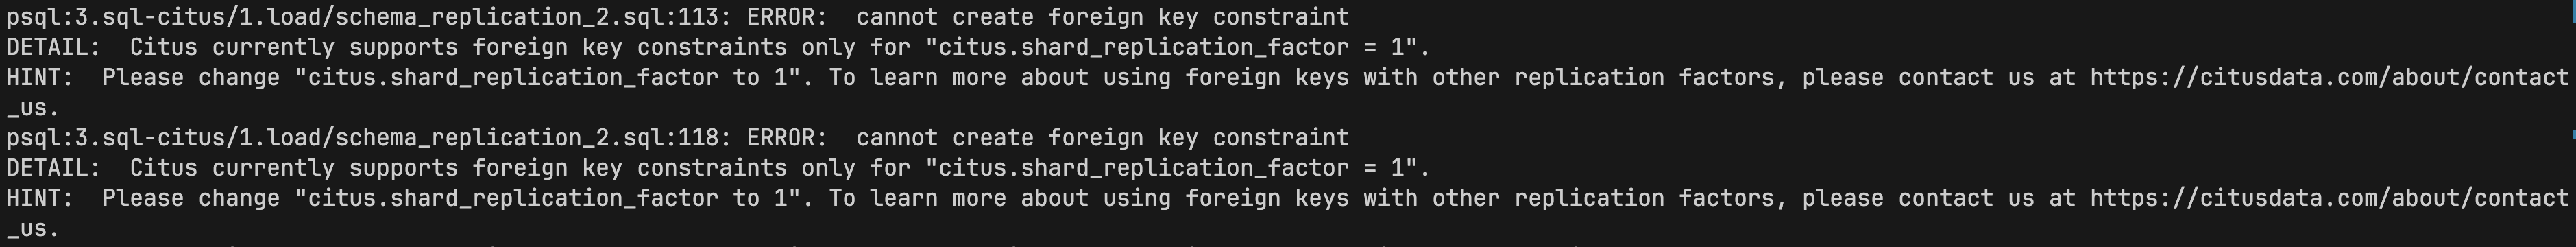
\includegraphics[width=\textwidth]{fotos/citus/shard_rep_foreign_key_errro.png}
\caption{Citus, error de clave foránea con replicación.}
\label{fig:citus_shard_factor}
\end{figure}

En la figura \ref{fig:citus_shard_factor}, podemos observar como Citus vuelve a quejarse de claves foráneas. Antes era capaz de manejar claves foráneas en una tabla distribuida siempre y cuando estas hicieran referencia a atributos de tablas de referencia o de tablas distribuidas y co-localizadas, una limitación que surge de la necesidad de los datos de claves foráneas a residir en el mismo nodo; sin embargo, al añadir la replicación de \textit{shards}, esta imposición es imposible de garantizar. \\

No obstante, no necesitamos modificar el código ya que las tablas se han creado correctamente, como indica la figura \ref{fig:citus_shard_table}. Únicamente la clave foránea no se ha creado, pero no existe manera de solucionar este inconveniente con la versión de Citus instalada, la última disponible.

\begin{figure}[H]
\centering
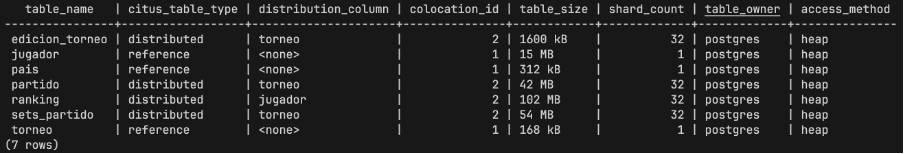
\includegraphics[width=0.7\textwidth]{fotos/citus/shard_tablas.png}
\caption{Citus, tablas con replicación.}
\label{fig:citus_shard_table}
\end{figure}

Procedemos ahora a parar uno de los nodos y comprobamos que sí podemos ejecutar las consultas (figura \ref{fig:citus_shard_query}), aunque Citus nos avisa de que no ha podido comunicarse con un nodo.

\begin{figure}[H]
\centering
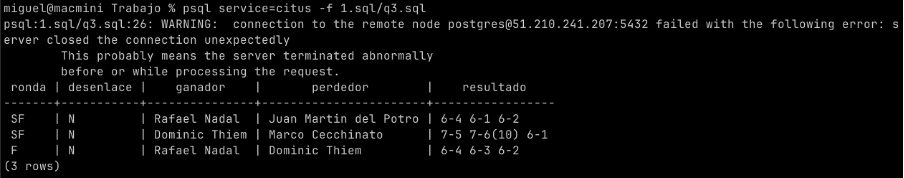
\includegraphics[width=0.7\textwidth]{fotos/citus/shard_consulta.png}
\caption{Citus, consulta a tabla distribuida con un nodo apagado.}
\label{fig:citus_shard_query}
\end{figure}

\subsection*{Citus Columnar}

El formato columnar de Citus introduce soporte para almacenamiento de datos en un formato columnar, diseñado para optimizar el rendimiento en cargas de trabajo analíticas, donde las consultas suelen procesar grandes volúmenes de datos pero acceden a unas pocas columnas específicas. El modo columnar permite una compresión más eficiente y reduce la cantidad de datos leídos. No obstante, las tablas con acceso columnar se convierten en \texttt{append only}, es decir, solo se pueden añadir nuevos datos, no se pueden hacer operaciones\texttt{UPDATE} o \texttt{DELETE}. \\

Para configurar una tabla con formato columnar, lo indicamos de la siguiente forma:

\begin{minted}[frame=single, fontsize=\footnotesize]{sql}
CREATE TABLE partido (
    torneo                  INT,
    fecha                   DATE,
     …
    PRIMARY KEY (torneo, fecha, num_partido)
) USING columnar;
\end{minted}


Una vez cargado el esquema, podemos inspeccionar la tabla \texttt{partido} y en la figura \ref{fig:citus_columnar} observamos que el método de acceso se ha modificado correctamente de \texttt{heap}, el valor por defecto, a \texttt{columnar}.

\begin{figure}[H]
\centering
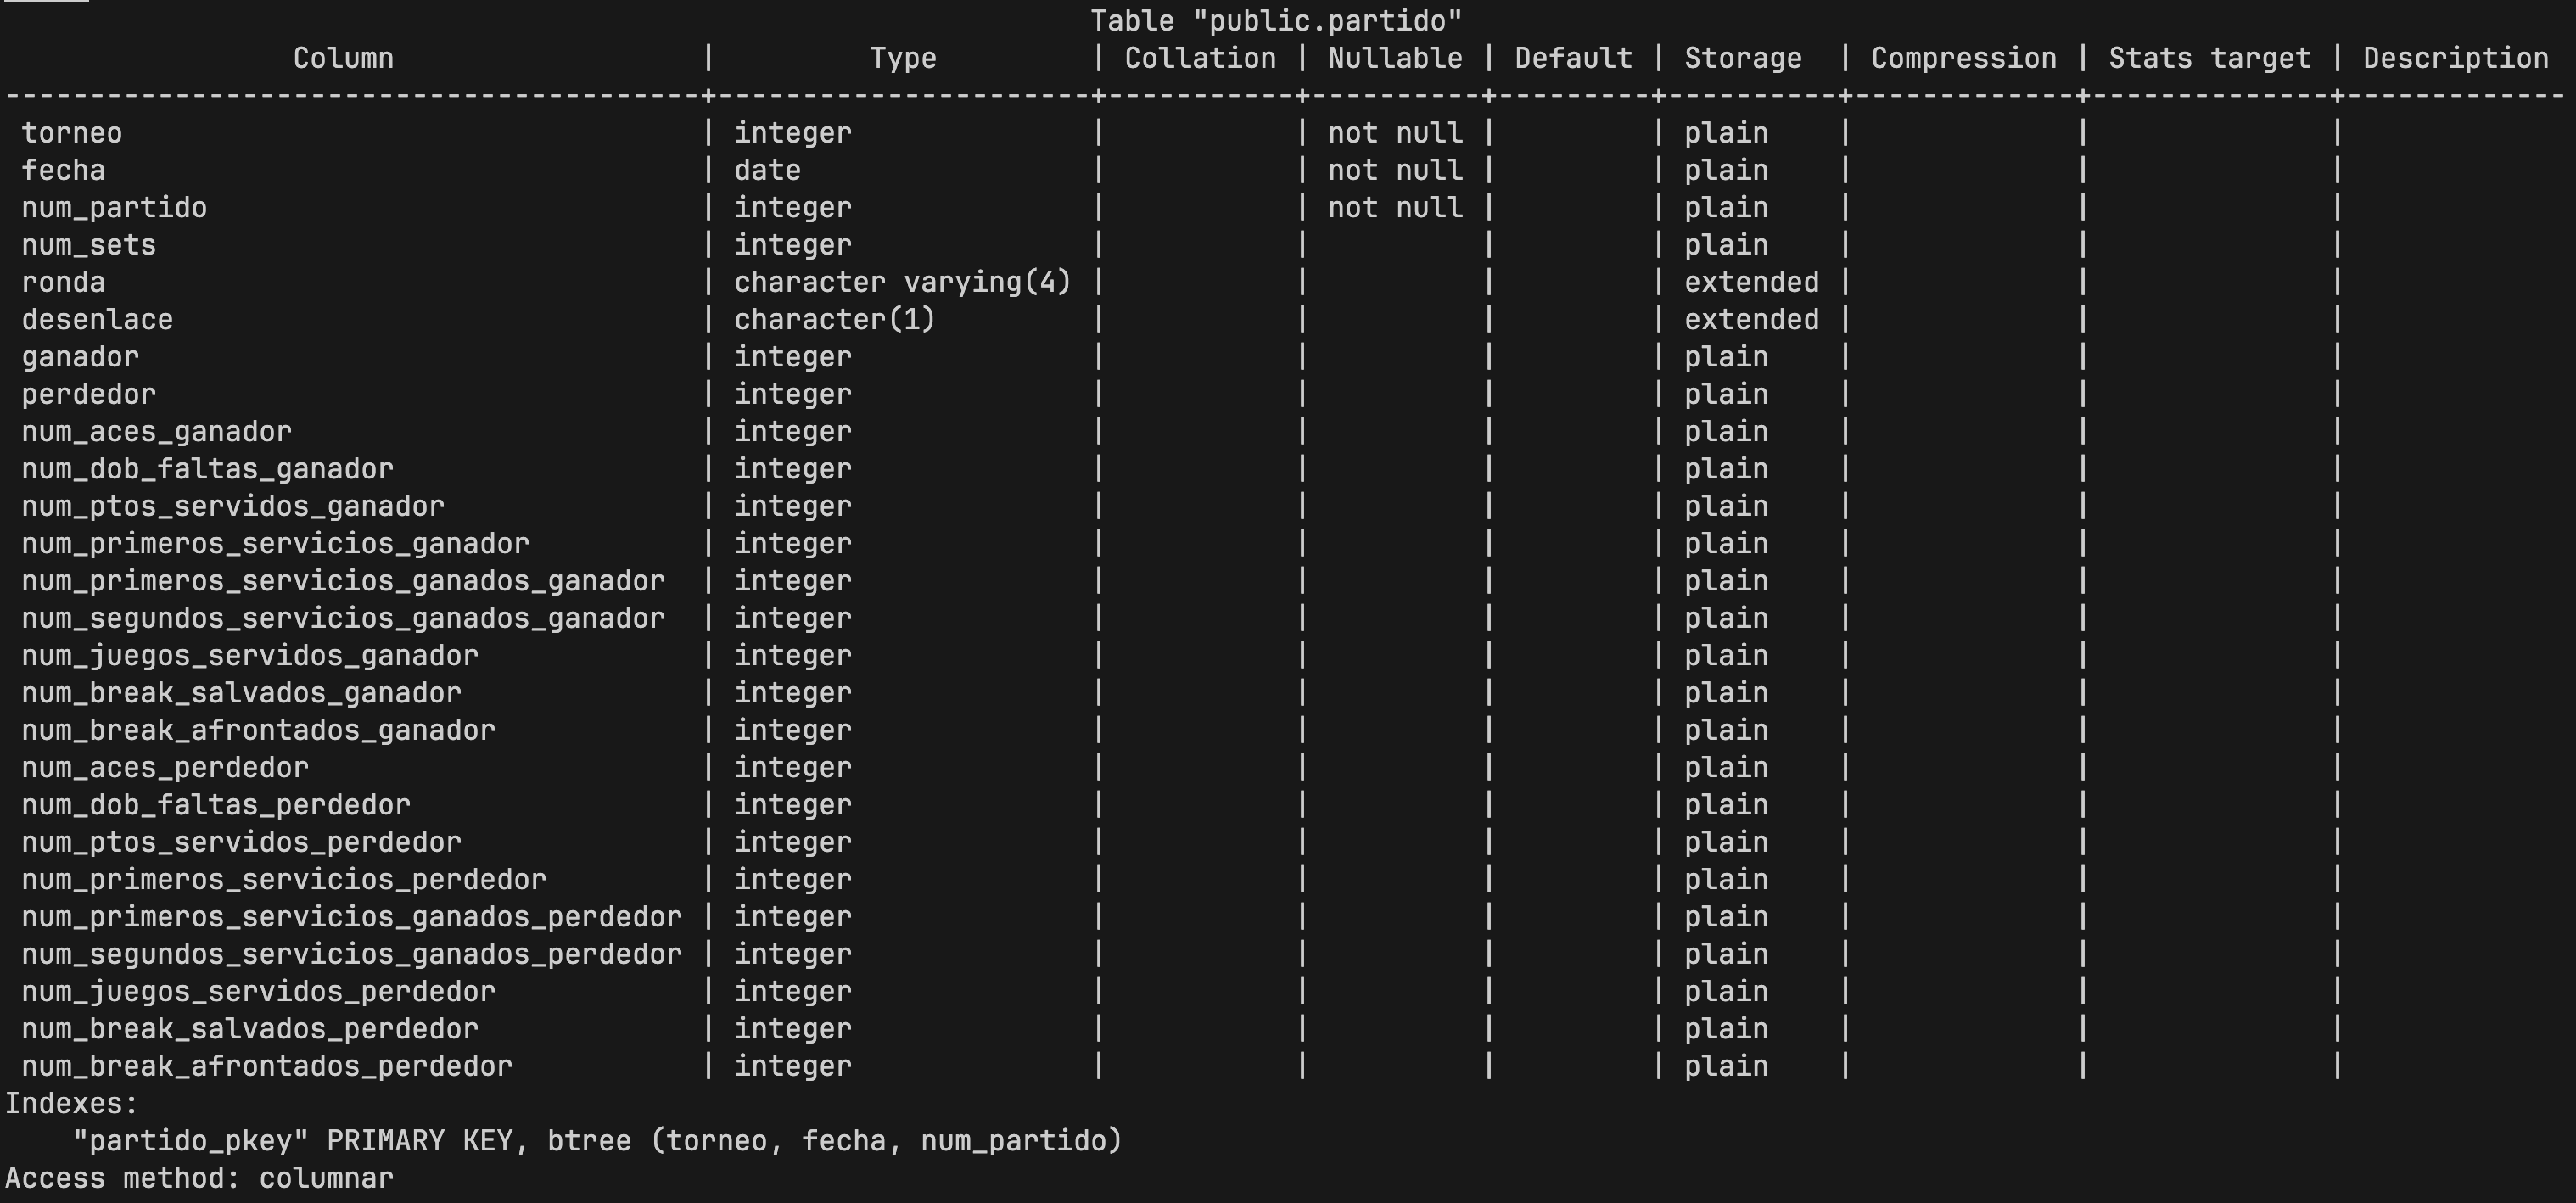
\includegraphics[width=\textwidth]{fotos/citus/detalle_partido_columnar.png}
\caption{Citus, tabla partido con acceso columnar.}
\label{fig:citus_columnar}
\end{figure}
\newpage

\subsection*{Comparación de tiempos}

Para medir el tiempo de ejecución de las consultas, se ha empleado el comando \textit{timing} en \texttt{psql} para obtener el tiempo de ejecución en milisegundos. Esto lo haremos desde el nodo coordinador del \textit{cluster} para reducir la latencia. \\

\begin{table}[H]
\centering
\begin{tabular}{cccccc}
\hline
 & Q1 [ms] & Q2 [ms] & Q3 [ms] & Q4 [ms] & Q5 [ms] \\
\hline\hline
\textbf{Row} & & & & & \\
\hline
Ejecución 1 & 29.354 & 42.19 & 32.146 & 169.904 & 90.101 \\
Ejecución 2 & 29.708 & 35.563 & 37.633 & 167.64 & 97.767 \\
Ejecución 3 & 33.938 & 38.538 & 36.29 & 134.863 & 131.97 \\
Ejecución 4 & 18.23 & 32.685 & 48.048 & 149.431 & 84.634 \\
Ejecución 5 & 21.41 & 33.993 & 29.891 & 146.508 & 72.72 \\ \hline
Media $\pm \sigma$ & 26.928 $\pm$ 5.88 & 36.994 $\pm$ 3.78 & 36.802 $\pm$ 6.59 & 153.669 $\pm$ 14.39 & 95.438 $\pm$ 20.93 \\ \hline\hline
\textbf{Columnar} & & & & & \\
\hline\hline
Ejecución 1 & 21.682 & 28.574 & 30.581 & 350.034 & 80.681 \\
Ejecución 2 & 13.919 & 22.264 & 31.815 & 358.8 & 48.361 \\
Ejecución 3 & 19.801 & 18.089 & 32.237 & 340.87 & 58.983 \\
Ejecución 4 & 13.919 & 20.912 & 32.962 & 358.214 & 92.353 \\
Ejecución 5 & 16.355 & 17.047 & 27.685 & 375.217 & 50.133 \\\hline
Media $\pm \sigma$ & 17.135 $\pm$ 3.133 & 21.377 $\pm$ 4.059 & 31.056 $\pm$ 1.854 & 356.627 $\pm$ 11.354 & 66.102 $\pm$ 17.448 \\
\hline
\end{tabular}
\caption{Citus, comparación de tiempos de ejecución (en milisegundos) de las diferentes consultas en tablas con acceso columnar frente a acceso por filas. Cada consulta se ejecutó 5 veces para sacar una estadística fiable.}
\label{fig:citus_tiempos}
\end{table}

Podemos observar en la tabla \ref{fig:citus_tiempos} como el formato de acceso columnar mejora ligeramente los tiempos de ejecución en las consultas Q1, Q2, Q3 y Q5 frente al acceso por filas, pero empeora significativamente los de la consulta Q4. \\

Hacer un \textit{benchmark} de bases de datos no es tarea fácil, y los resultados pueden no reflejar los tiempos de ejecución reales en producción. Intentamos explicar los resultados obtenidos destacando que la consulta Q4 accede a muchas columnas de la tabla partidos para calcular las estadísticas de los jugadores, y este tipo de consultas, el tener que recuperar muchas columnas dentro de una fila, es uno de los puntos débiles de las tablas columnares, que destacan en tareas de agregación o en lecturas de pocas columnas de tablas grandes.
